\documentclass[11pt,letterpaper]{article}
\usepackage[top=3cm, bottom=2cm, left=2cm, right=2cm, columnsep=20pt]{geometry}
\usepackage{pdfpages}
\usepackage{graphicx}
\usepackage{etoolbox}
\apptocmd{\sloppy}{\hbadness 10000\relax}{}{}
% \usepackage[numbers]{natbib}
\usepackage[T1]{fontenc}
\usepackage{ragged2e}
\usepackage[french]{babel}
\usepackage{listings}
\usepackage{color}
\usepackage{soul}
\usepackage[utf8]{inputenc}
\usepackage[export]{adjustbox}
\usepackage{caption}
\usepackage{amsmath}
\usepackage{amssymb}
\usepackage{float}
\usepackage{csquotes}
\usepackage{fancyhdr}
\usepackage{wallpaper}
\usepackage{siunitx}
\usepackage[indent]{parskip}
\usepackage{textcomp}
\usepackage{gensymb}
\usepackage{multirow}
\usepackage[hidelinks]{hyperref}
\usepackage{abstract}
\usepackage{svg}
\usepackage{biblatex}
\addbibresource{bibliographie.bib}

\renewcommand{\abstractnamefont}{\normalfont\bfseries}
\renewcommand{\abstracttextfont}{\normalfont\itshape}
\usepackage{titlesec}
\titleformat{\section}{\large\bfseries}{\thesection}{1em}{}
\titleformat{\subsection}{\normalsize\bfseries}{\thesubsection}{1em}{}
\titleformat{\subsubsection}{\normalsize\bfseries}{\thesubsubsection}{1em}{}

\usepackage{xcolor}
\definecolor{codegreen}{rgb}{0,0.6,0}
\definecolor{codegray}{rgb}{0.5,0.5,0.5}
\definecolor{codepurple}{rgb}{0.58,0,0.82}
\definecolor{backcolour}{rgb}{0.95,0.95,0.92}
\lstdefinestyle{mystyle}{
    backgroundcolor=\color{backcolour},   
    commentstyle=\color{codegreen},
    keywordstyle=\color{magenta},
    numberstyle=\tiny\color{codegray},
    stringstyle=\color{codepurple},
    basicstyle=\ttfamily\footnotesize,
    breakatwhitespace=false,         
    breaklines=true,                 
    captionpos=b,                    
    keepspaces=true,                 
    numbers=left,                    
    numbersep=5pt,                  
    showspaces=false,                
    showstringspaces=false,
    showtabs=false,                  
    tabsize=2
}
\lstset{style=mystyle}

\usepackage[most]{tcolorbox}
\newtcolorbox{note}[1][]{
  enhanced jigsaw,
  borderline west={2pt}{0pt}{black},
  sharp corners,
  boxrule=0pt, 
  fonttitle={\large\bfseries},
  coltitle={black},
  title={Note:\ },
  attach title to upper,
  #1
}

%----------------------------------------------------

\setlength{\parindent}{0pt}
\DeclareCaptionLabelFormat{mycaptionlabel}{#1 #2}
\captionsetup[figure]{labelsep=colon}
\captionsetup{labelformat=mycaptionlabel}
\captionsetup[figure]{name={Figure }}
\newcommand{\inlinecode}{\normalfont\texttt}
\usepackage{enumitem}
\setlist[itemize]{label=\textbullet}

\begin{document}
\begin{titlepage}
\center

\begin{figure}
    \ThisULCornerWallPaper{.4}{Polytechnique_signature-RGB-gauche_FR.png}
\end{figure}
\vspace*{2 cm}

\textsc{\Large \textbf{PHS3910 --} Techniques expérimentales et instrumentation}\\[0.5cm]
\large{\textbf{Équipe : Lundi 03}}\\[1.5cm]

\rule{\linewidth}{0.5mm} \\[0.5cm]
\Large{\textbf{Spectromètre}} \\[0.2cm]
\text{Fiche technique}\\
\rule{\linewidth}{0.2mm} \\[2.3cm]

\large{\textbf{Présenté à}\\
  Jean Provost\\
  Lucien Weiss\\[2.5cm]
  \textbf{Par :}\\
  Émile \textbf{Guertin-Picard} (2208363)\\
  Philippine \textbf{Beaubois} (2211153)\\
  Marie-Lou \textbf{Dessureault} (2211129)\\
  Maxime \textbf{Rouillon} (2213291)\\[3cm]}

\large{\today\\
Département de Génie Physique\\
Polytechnique Montréal\\}

\end{titlepage}

%----------------------------------------------------

\tableofcontents
\pagenumbering{roman}
\newpage

\pagestyle{fancy}
\setlength{\headheight}{14pt}
\renewcommand{\headrulewidth}{0pt}
\fancyfoot[R]{\thepage}

\pagestyle{fancy}
\fancyhf{}
\renewcommand{\headrulewidth}{1pt}
\fancyhead[L]{\textbf{PHS3910}}
\fancyhead[C]{Fiche technique des spectromètres}
\fancyhead[R]{\today}
\fancyfoot[R]{\thepage}

\pagenumbering{arabic}
\setcounter{page}{1}

%----------------------------------------------------

\section{Description générale et spécifications}

\begin{figure}[H]
  \centering
  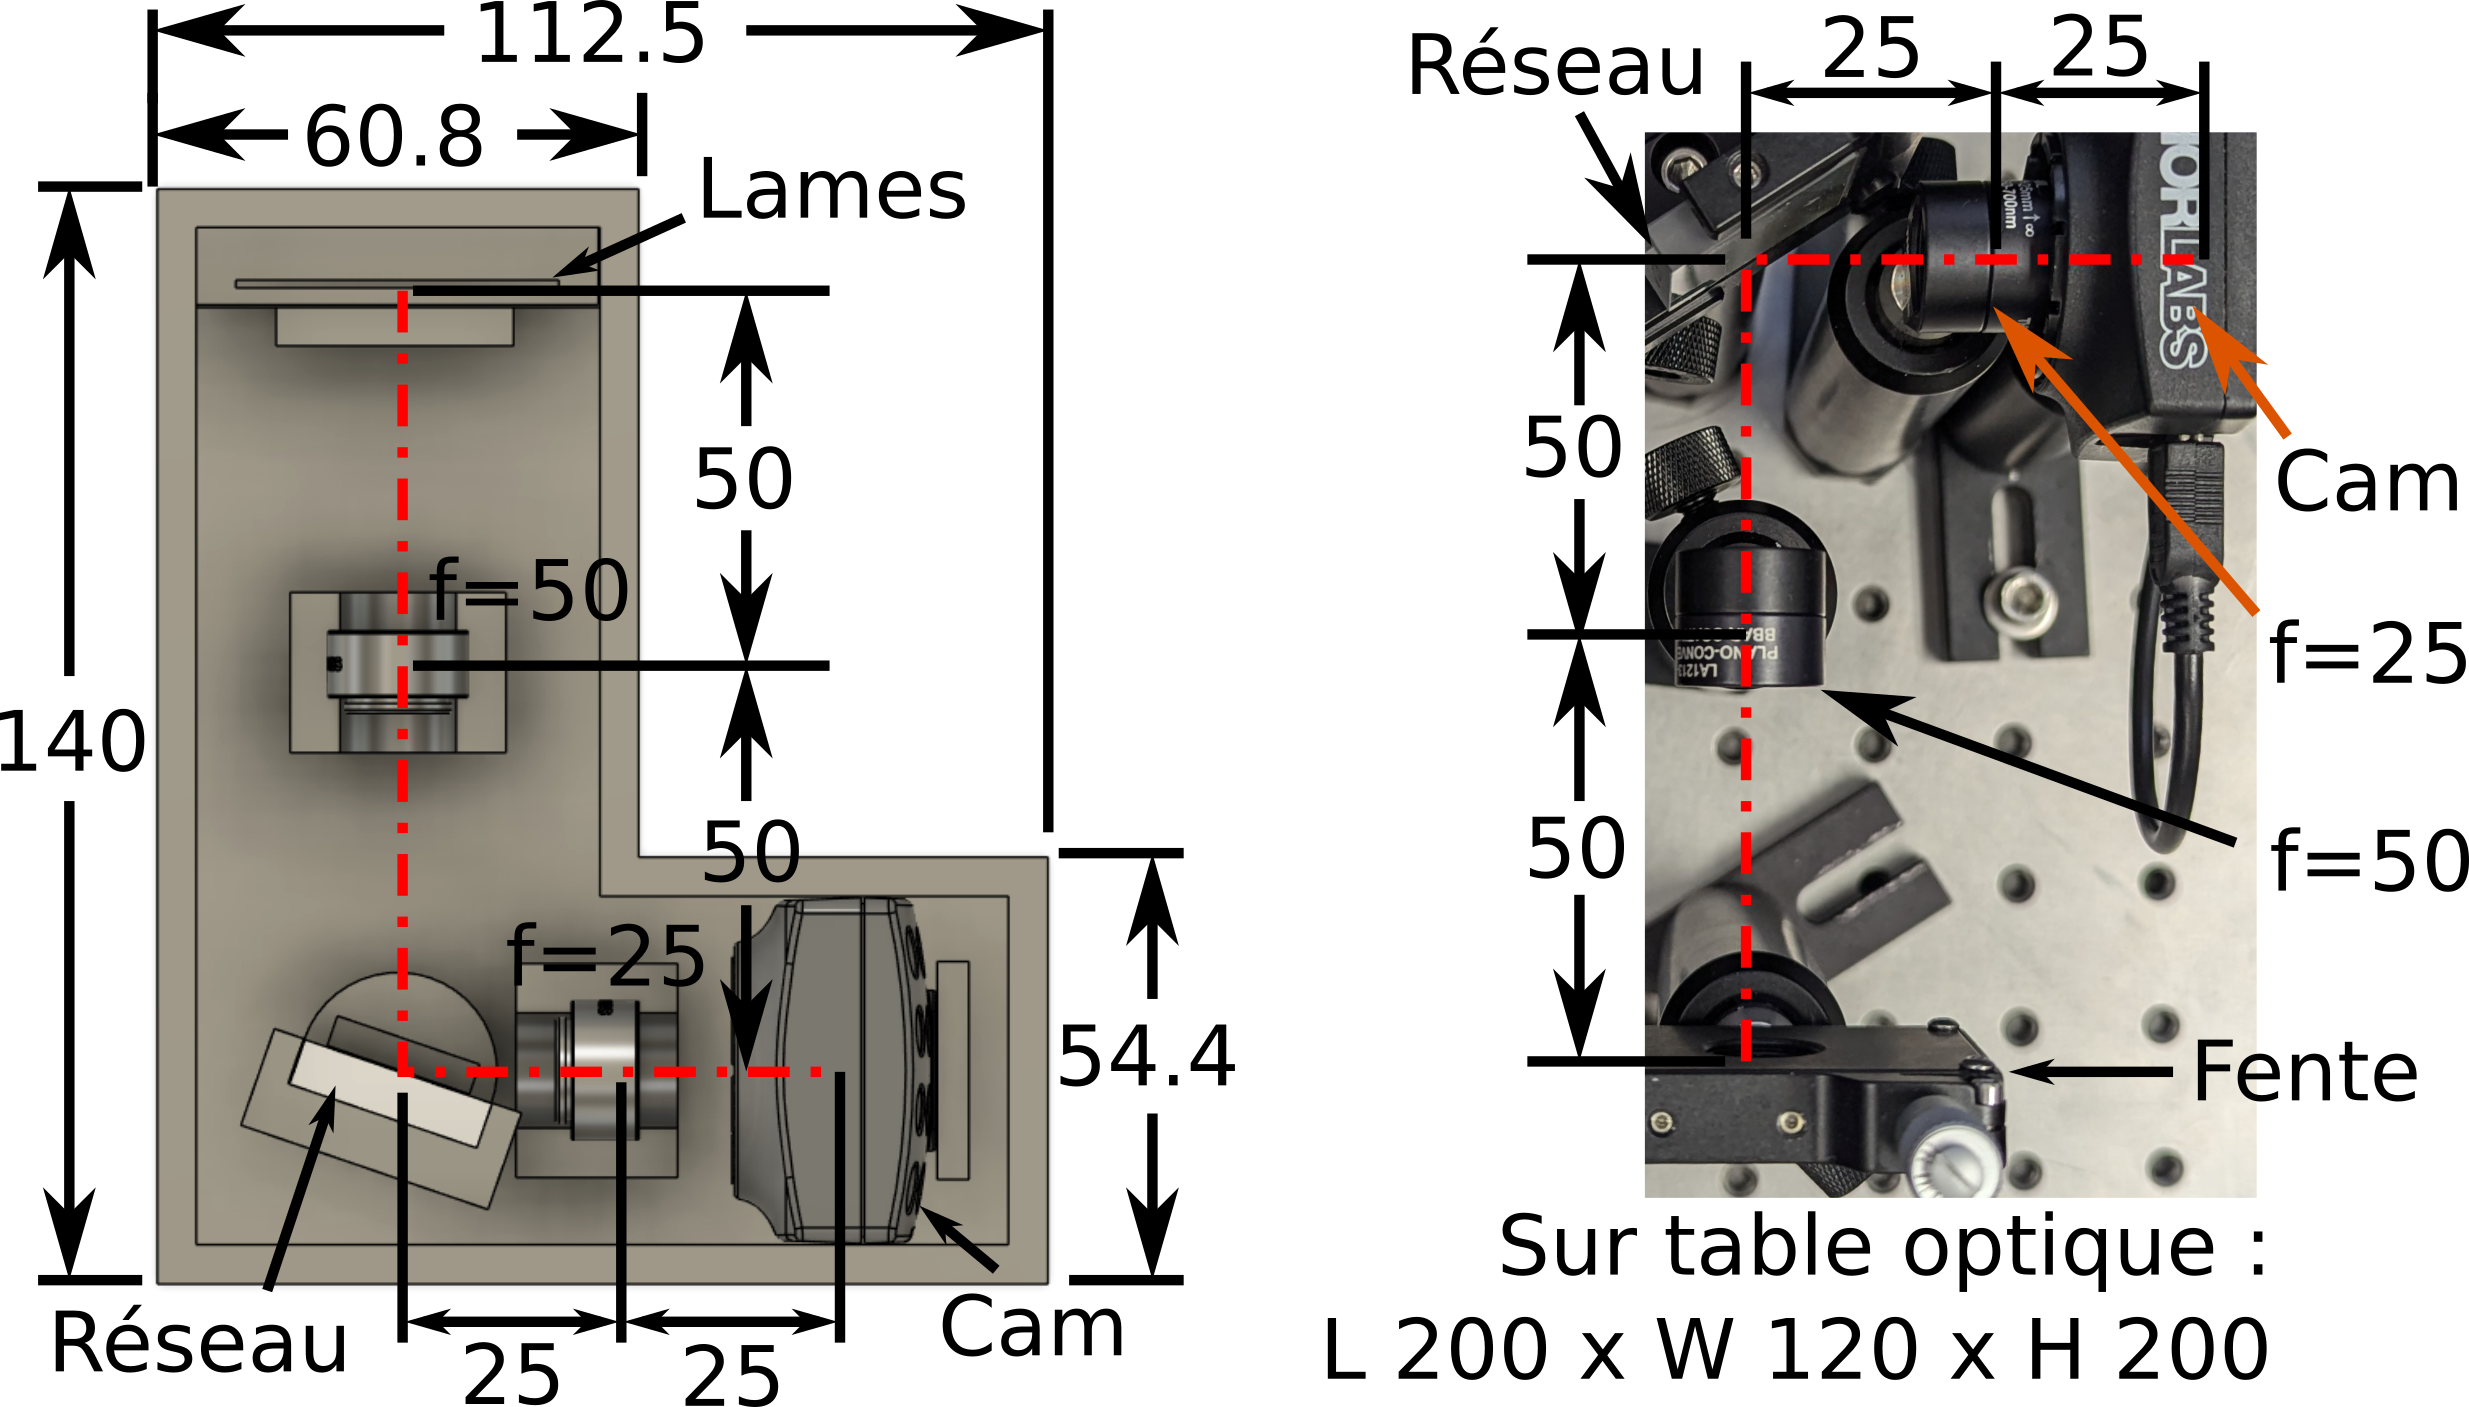
\includegraphics[scale=1.75]{schema_spectros.png}
  \caption{test}
  \label{test}
\end{figure}


\section{test tableaux}

\begin{table}[!ht]
    \centering
    \caption{Liste des pièces et coûts totaux pour le spectromètre sur table optique}
    \begin{tabular}{|l|l|c|r|r|}
    \hline
        ID pièce & Description & Qté & \$ CAD & Total ind. \\ \hline\hline
        LA-1560-A-ML & Lentille plano-convexe f=25 mm & 1 & \$72.25 & \$72.25 \\ \hline
        LA-1213-A-ML & Lentille plano-convexe f=50 mm & 1 & \$70.61 & \$70.61 \\ \hline
        NE506A & Filtre atténuateur de lumière & 2 & \$59.55 & \$119.10 \\ \hline
        GR25-0605 & Réseau de diffraction 600/mm & 1 & \$178.32 & \$178.32 \\ \hline
        DCC1545M-GL & Caméra USB & 1 & \$539.21 & \$539.21 \\ \hline
        VA100 & Fente ajustable & 1 & \$417.74 & \$417.74 \\ \hline
        KM100S & Montage à réseau de diffraction & 1 & \$130.45 & \$130.45 \\ \hline
        SMR05 & Trou taraudé pour lentilles & 2 & \$28.68 & \$57.35 \\ \hline
        TR3-P5, & 5 tiges pour optiques & 1 & \$38.50 & \$38.50 \\ \hline
        BA1 & Pied de montage optique & 2 & \$8.42 & \$16.85 \\ \hline
        BA1S & Pied de montage optique & 4 & \$7.83 & \$31.30 \\ \hline
        PH6 & Base pour tiges d'optique & 5 & \$20.43 & \$102.17 \\ \hline
        PH4 & Base pour tiges d'optique & 1 & \$14.83 & \$14.83 \\ \hline
        VC1 & Pince en V & 1 & \$64.04 & \$64.04 \\ \hline\hline
        ~ & ~ & ~ & Total : & \$1,852.72 \\ \hline
    \end{tabular}
    \label{prix_table}
\end{table}

\begin{table}[!ht]
    \centering
    \caption{Liste des pièces et coûts totaux pour le spectromètre avec impression 3D}
    \begin{tabular}{|l|l|c|r|r|}
    \hline
        ID pièce & Description & Qté & \$ CAD & Total ind. \\ \hline\hline
        LA-1560-A-ML & Lentille plano-convexe f=25 mm & 1 & \$72.25 & \$72.25 \\ \hline
        LA-1213-A-ML & Lentille plano-convexe f=50 mm & 1 & \$70.61 & \$70.61 \\ \hline
        GR25-0605 & Réseau de diffraction 600/mm & 1 & \$178.32 & \$178.32 \\ \hline
        DCC1545M-GL & Caméra USB & 1 & \$539.21 & \$539.21 \\ \hline
        - & Impression 3D & 1 & \$6.94 & \$6.94 \\ \hline
        - & Ensemble de lames de rasoir & 1 & \$9.95 & \$9.95 \\ \hline\hline
        ~ & ~ & ~ & Total : & \$877.28 \\ \hline
    \end{tabular}
    \label{prix_3D}
\end{table}

% \clearpage
% \printbibliography
% \bibliographystyle{unsrtnat}
% \bibliography{My_Library}

\end{document}
